\documentclass{article}
\usepackage[utf8]{inputenc}
\usepackage{graphicx}
\usepackage[spanish,es-tabla]{babel}
\usepackage{amsmath}
\usepackage[a4paper,margin=1in]{geometry}
\usepackage{subcaption}
\usepackage{amssymb}
\usepackage{amsmath}
\usepackage[hidelinks]{hyperref}
\usepackage{mathtools}
\usepackage[table,xcdraw]{xcolor}
\usepackage[backend=bibtex]{biblatex}
\usepackage{csquotes}
\usepackage[spanish]{babel}
\usepackage[utf8]{inputenc} %Este paquete permite poner acentos directamente y ees
\usepackage{fontenc}
\usepackage{circuitikz}
\usepackage{amsmath}
\usepackage{graphicx}%[pdftex]
\usepackage{graphicx, wrapfig}
\usepackage{fancyhdr}
\usepackage{anysize}
\usepackage{verbatim}
\usepackage{advdate}
\usepackage{colortbl}
\usepackage{amsmath}
\usepackage{amssymb}
\usepackage[dvips,final]{epsfig}
\usepackage{epstopdf}
\usepackage{hyperref}
\usepackage{enumitem}
\usepackage{siunitx}
\usepackage[english]{babel}
\usepackage{sectsty}
\usepackage{array}
\usepackage{listings}
\usepackage{empheq}
\usepackage{minted}
\usepackage{xcolor}
\usepackage[spanish]{babel}
\marginsize {2.5cm}{2.5cm}{2.5cm}{2.5cm} %Primero margen izquierdo, Segundo margen derecho, Tercero margen superior, Cuarto margen inferior.
\usepackage{float}
\usepackage{fancyhdr}
\addbibresource{bibliografia.bib} %archivo de bibliografia

\begin{document}

\pagestyle{fancy}
\fancyhf{}
\fancyhead[L]{Trabajo práctico N°2 - Electrónica Analógica 3}
\fancyfoot[L,RO]{\thepage}
\fancyfoot[LO]{}
\renewcommand{\footrulewidth}{0.1pt}


\renewcommand{\figureautorefname}{Fig.}
\renewcommand{\tableautorefname}{Tab.}
\renewcommand{\equationautorefname}{Ec.}

\begin{titlepage}

\thispagestyle{empty}

% Portada Custom, ver /maketitle: https://www.overleaf.com/learn/latex/How_to_Write_a_Thesis_in_LaTeX_(Part_5)%3A_Customising_Your_Title_Page_and_Abstract


\begin{center}
    
\includegraphics[width=5cm]{figures/unc_logo.png} \hspace{2cm}
    
\includegraphics[width=5cm]{figures/fcefyn_logo.jpg}
    \\[1cm]
    \vspace{5pt}
    \LARGE Universidad Nacional de Córdoba\\[0.5cm] 
    \large Facultad de Ciencias Exactas, Físicas y Naturales \\[0.5cm] 
    \large Electrónica Analógica III
    \\[0.2cm]
    \large Trabajo Práctico N° 2
    \\[0.2cm]
    \vspace{60pt}
    \begin{table}[!h]
    \centering
    \begin{tabular}{ll}
    \multicolumn{1}{c}{Nombre} & \multicolumn{1}{c}{DNI} \\
    Nicolás Gallardo & 42.218.184 \\
    Jeremías Clemenz & 43.449.566 \\
    Facundo Rodriguez & xx.xxx.xxx \\
    
    \end{tabular}
    \end{table}
    \vspace{20pt}
    \begin{table}[!h]
    \centering
    \begin{tabular}{ll}
    \multicolumn{1}{c}{Docentes} & Ing. Rodrigo Bruni \\
     & Ing. José Amado \\
     & Ing. Federico Dadam
    \end{tabular}
    \end{table}
    \vfill
    Córdoba, República Argentina\\
    \today
\end{center}

\end{titlepage}
\newpage

\tableofcontents
\newpage
\listoffigures
\newpage
\listoftables

\newpage

\section{Introducción}

\hspace{1mm} En este trabajo practico, se busca comprender, diseñar e implementar un amplificador clase A en RF. Debido a que en RF, las longitudes de onda son del orden de los componentes que se utilizan típicamente, como resistencias, capacitores, etc. lo que imposibilita la utilización de los parámetros concentrados. Por lo tanto, se utiliza el concepto de parámetros distribuidos para diseñar el circuito mediante microtiras.

\section{Marco teórico}
\hspace{1mm} Los parámetros distribuidos se utilizan en RF para modelar y comprender el comportamiento de las señales a lo largo de las lineas de transmisión. La tensión y corriente comienzan a depender de la posición y del tiempo. %revisar
Esto hace que estos sean complejos de medir, debido a que según la posición en donde se coloque el instrumento de medición, la medición seria distinta. Uno de los modelos de parámetros concentrados mas utilizados son los Z, donde estos representan las impedancias de una determinada red. Para poder calcular los parámetros Z se debe realizar un cortocircuito o circuito abierto según corresponda, ya sea en la entrada o la salida. Realizar esto en alta frecuencia es complicado, por lo que no resulta una opción utilizar parámetros concentrados.
Es por esto que se utilizan  RF se utilizan los parámetros distribuidos, para modelar y comprender el comportamiento de las señales a lo largo de las lineas de transmisión,
Un circuito resonante LC está compuesto por un inductor L y un capacitor CT, estos se conectan como se observa en la figura 1.

\begin{figure}[!h]
    \centering
    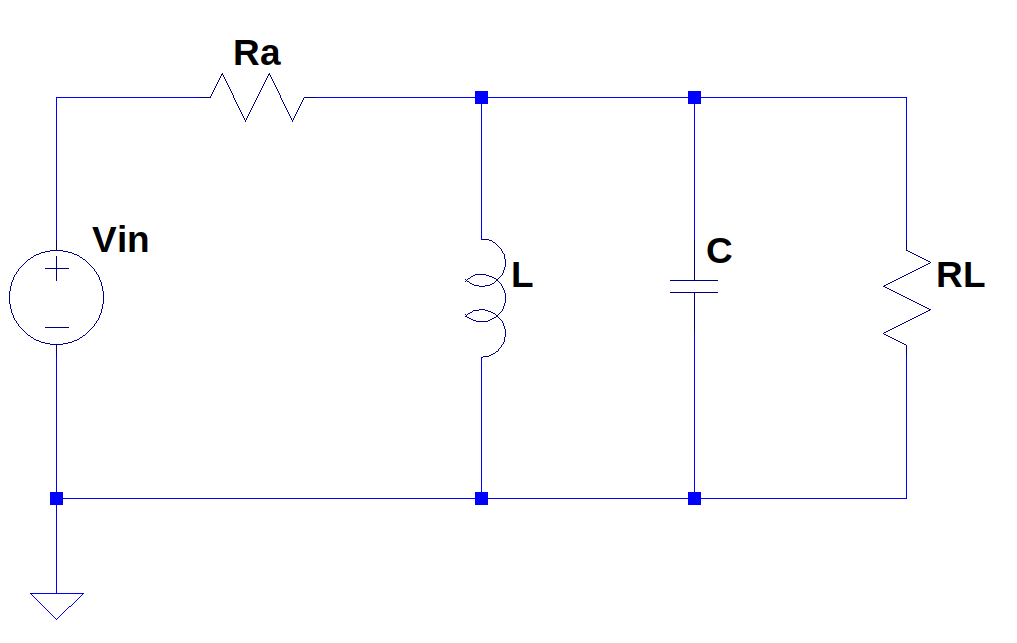
\includegraphics[width=0.8\textwidth]{Imagenes/LC.png}
    \caption{Circuito LC}
    \label{fig:LC}
\end{figure}

\hspace{1mm} Este circuito va a tener una frecuencia de resonancia donde la misma se encuentra mediante la siguiente ecuación:

\begin{equation}
    f_o = \frac{1}{2\pi \sqrt{LC}}
\end{equation}

\hspace{1mm} Por lo tanto, hay múltiples combinaciones de \(L\) y \(C\) para una determinada frecuencia de resonancia.
Otro parámetro importante en estos circuitos, es el factor de calidad \(Q\), para este circuito se analizan dos factores de calidad. Por un lado, el factor de calidad cargado \( Q_{\text{c}} \) el cual tiene sentido cuando la carga está conectada al circuito resonante, mientras que el descargado \( Q_{\text{d}} \) cuando el circuito no tiene carga. Las ecuaciones de estos parámetros son las siguientes:

\begin{equation}
    Q_d = \frac{R_p}{X_L} 
\end{equation}

\begin{equation}
    Q_c = \frac{fo}{BW} = \frac{R_T}{X_L}
\end{equation}

%Siendo:
%\begin{equation}
%   R_T = R_a//R_p//R_L
%\end{equation}
\newpage
Donde:
\begin{itemize}
    \item \( f_o \) es la frecuencia de resonancia,
    \item \( BW \) es el ancho de banda del circuito,
    \item \( R_T \) es la resistencia total del circuito,
    \item \( R_a \) es la resistencia del generador,
    \item \( R_p \) es la resistencia parásita del inductor
    \item \( R_L \) es la resistencia de carga del circuito, y
    \item \( X_L \) es la reactancia inductiva. 
    
\end{itemize}

Es evidente, que si se tiene una frecuencia de resonancia dada y deseáramos definir el ancho de banda, el valor de las resistencias que componen a \( R_T \), tanto \( R_a \) como  \( R_L \) no se podrían modificar debido a que son valores fijos y \( R_p \) depende del diseño de la bobina. Por lo tanto, se plantea una forma de solucionar dicho inconveniente, modificando el hecho de tener un solo capacitor total \(C_T\), a tener 4 capacitores que en conjunto sigan siendo equivalentes a \(C_T\), lo que resulta en que \( f_o \) no se modifica. Lo siguiente es que la entrada como la salida se conecten al punto medio para con esto, poder plantear un modelo equivalente mucho mas sencillo de analizar al reflejar \( R_a \) y \( R_L \) y de esta forma todas las resistencias queden en paralelo a \( R_p \).

\begin{figure}[!h]
    \centering
    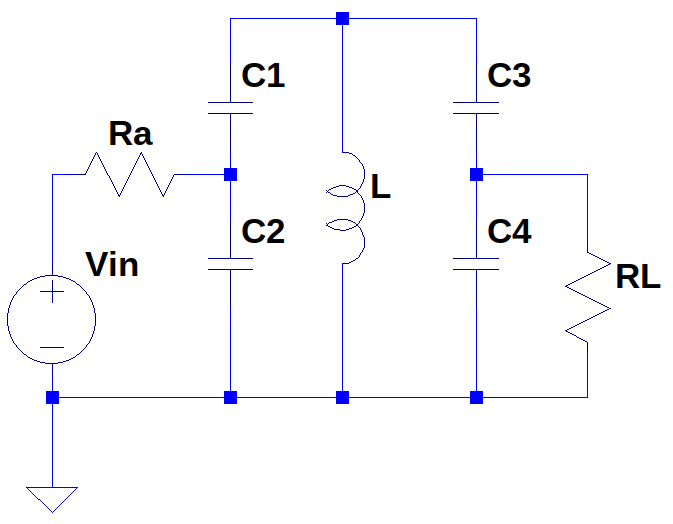
\includegraphics[width=0.8\textwidth]{Imagenes/LC_2.png}
    \caption{Circuito LC con 4 capacitores}
    \label{fig:LC_2}
\end{figure}

Para que \( f_o \) se mantenga en el mismo valor, los capacitores deben cumplir la siguiente ecuación:  

\begin{equation}
    \frac{C_T}{2} = \frac{C_1C_2}{C_1+C_2} = \frac{C_3C_4}{C_3+C_4}
\end{equation}
Luego, para reflejar las resistencias, se utiliza el concepto de un autotransformador:
\begin{figure}[!h]
    \centering
    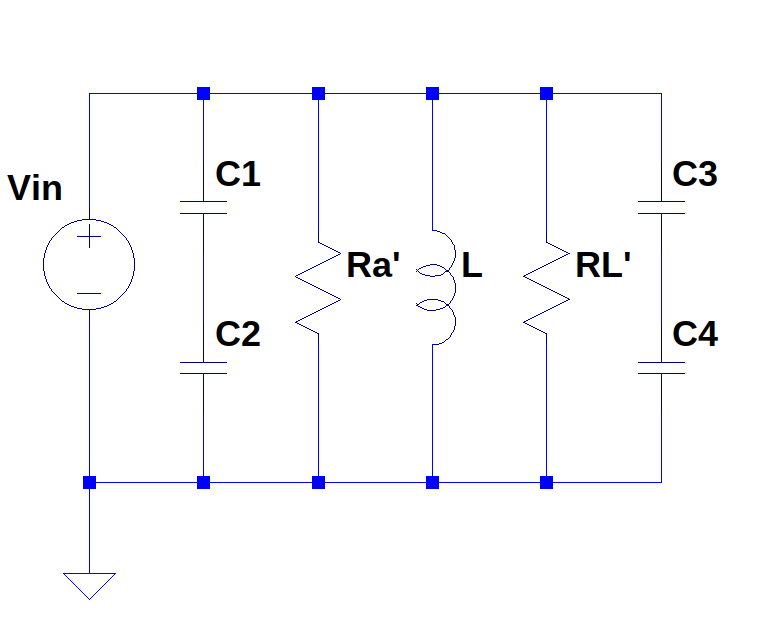
\includegraphics[width=0.8\textwidth]{Imagenes/LC_3.png}
    \caption{Circuito LC reflejado}
    \label{fig:LC_3}
\end{figure}
\begin{equation}
    R_a' = (1+\frac{C_2}{C_1})^2R_a
\end{equation}

\begin{equation}
    R_L' = (1+\frac{C_4}{C_3})^2R_L
\end{equation}

Por lo tanto,
\begin{equation}
    R_T = R_a'//R_p//R_L' 
\end{equation}

Finalmente, se deben cumplir las siguientes ecuaciones:

\begin{equation}
    2R_T = (R_L'//R_p) 
\end{equation}

\begin{equation}
    2R_T = R_a' 
\end{equation}

Para que de esta forma, el paralelo de la ecuación (8) y (9) resulten en \(R_T\) 
\newpage
\subsection{Redes L}
Esta se trata de uno de los acoplamientos de impedancias mas sencillos, esta compuesta por un inductor y un capacitor, justamente en una disposición en forma de L. Se tienen 4 configuraciones típicas:
\begin{minipage}{0.5\textwidth}
% Circuito L serie pasa bajo
\begin{circuitikz}

    % Generador de RF
    \draw (0,0) to[sV,l=$V_g$] (0,2);
    % Resistencia en serie
    \draw (0,2) to[R,l=$R_g$] (2,2);
    % Red L pasa bajo
    \draw (2,2) to[C,l=$C$] (2,0) ;
    \draw (2,2) to[L,l=$L$] (4,2) ;
    % Carga RL
    \draw (4,2) to[R,l=$R_L$] (4,0);
    \draw (0,0) -- (4,0);
\end{circuitikz}
\captionof{figure}{Filtro pasa bajo}
\end{minipage}
\begin{minipage}{0.5\textwidth}
% Circuito L paralelo pasa bajo
\begin{circuitikz}
    % Generador de RF
    \draw (0,0) to[sV,l=$V_g$] (0,2);
    % Resistencia en serie
    \draw (0,2) to[R,l=$R_g$] (2,2);
    % Red L pasa bajo
    \draw (2,2) to[L,l=$L$] (2,0);
    \draw (2,2) to[C,l=$C$] (4,2);
    % Carga RL
    \draw (4,2) to[R,l=$R_L$] (4,0);
    \draw (0,0) -- (4,0);
\end{circuitikz}
\captionof{figure}{Filtro pasa alto}
\end{minipage}
\begin{minipage}{0.5\textwidth}

% Circuito L serie pasa alto
\begin{circuitikz}
    % Generador de RF
    \draw (0,0) to[sV,l=$V_g$] (0,2);
    % Resistencia en serie
    \draw (0,2) to[R,l=$R_g$] (2,2);
    % Red L pasa alto
    \draw (2,2) to[C,l=$C$] (4,2) to[L,l=$L$] (4,0);
    % Carga RL
    \draw (5,2) to[R,l=$R_L$] (5,0);
    \draw (0,0) -- (5,0);
    \draw (4,2) -- (5,2);
\end{circuitikz}
\captionof{figure}{Filtro pasa alto}
\end{minipage}
\begin{minipage}{0.5\textwidth}
% Circuito L paralelo pasa alto

 \begin{circuitikz}
    % Generador de RF
    \draw (0,0) to[sV,l=$V_g$] (0,2);
    % Resistencia en serie
    \draw (0,2) to[R,l=$R_g$] (2,2);
    % Red L pasa alto
    \draw (2,2) to[L,l=$L$] (4,2) to[C,l=$C$] (4,0);
    % Carga RL
    \draw (5,2) to[R,l=$R_L$] (5,0);
    \draw (0,0) -- (5,0);
    \draw (4,2) -- (5,2);
\end{circuitikz}
\captionof{figure}{Filtro pasa bajo}
\end{minipage}

\bigskip

Estas, se utilizan según la relación de las impedancias, si se busca adaptar las impedancias porque la de entrada es mayor que la de salida, se utilizan los circuitos de la figura 4 y 5, mientras que si la impedancia de entrada es menor que la de salida se utilizan los de la figura 6 y 7. Si analizamos el caso del acoplamiento del circuito visto en este trabajo practico, se tiene que la $R_g=50\Omega$ y $R_L=1k\Omega$, si se tuviera que adaptar dichas impedancias se debería utilizar la configuración de la figura 6 o 7, se utilizara la figura 7.
Las ecuaciones que se utilizan para el diseño de dicho circuito son las siguientes:
\begin{equation}
\begin{aligned}
& X_L=\sqrt{R_g R_L-R_g^2} \\
& Q=\sqrt{\frac{R_L}{R_g}-1} \\
& X_c=\frac{R_g R_L}{X_L}   \\
& C = \frac{1}{2\pi f X_c} \\
& L = \frac{X_L}{2\pi f}
\end{aligned}
\end{equation}
De esta forma, teniendo la frecuencia de resonancia $f_o$ y utilizando los valores de $X_L$ y $X_c$ se calculan los valores del capacitor e inductor del circuito.
\newpage

\section{Diseño}

\subsection{Especificaciones del circuito}
\bigskip
Se plantea un circuito con las siguientes características
\begin{itemize}
    \item \( f_o = 14 \, \) MHz
    \item \( Q_c = 10 \) 
    \item \( R_a = 50 \) $\Omega$
    \item \( R_L = 1 \) K$\Omega$ 
\end{itemize}

\subsection{Diseño del inductor}
Para el diseño de la bobina se realizó una tabla en Excel, donde se utilizó la siguiente ecuación:

\begin{equation}
    L = D^3 N_s^2 k \times 10^{-3} \, \mu \text{Hy}
\end{equation}

Donde:
\begin{itemize}
    \item \( D\, \) es el diámetro externo de la bobina, su unidad es en centímetros.
    \item \( N_s \) es el numero de espiras por unidad de longitud, su unidad es vueltas por centímetro.
    \item \( k\) es el factor de Nagaoka.
\end{itemize}
Con la ecuación (11) obtenemos el valor de la inductancia de la bobina. También debemos recordar otras variables que están implícitas dentro de la misma.
\begin{equation}
    N_s = \frac{N}{\ell} = \frac{1}{p} = \frac{1}{S_e+d}
\end{equation}
Donde:
\begin{itemize}
    \item \( N\, \) es el número de espiras, en vueltas.
    \item \( \ell\, \) es la longitud del inductor, en centímetros.
    \item \( p\, \) es el paso, en centímetros.
    \item \( S_e \) es la separación entre espiras, en centímetros. 
    \item \( d\) es el diámetro del conductor, en centímetros.
\end{itemize}

Para comenzar, se deben fijar algunos de estos parámetros. Se definen los siguientes:
\begin{itemize}
    \item \( D = 2 \, \) cm 
    \item \( d = 0,1 \, \) cm 
    \item \( S_e = 0,1 \) cm
\item \( \ell = 3 \) cm
\end{itemize}
Con esto, podemos calcular el factor de Nagaoka a través de las curvas, ingresando con \(\frac{\ell}{D}=1,5\) el cual resulta aproximadamente en \(k = 11,5\).
\newpage
\begin{figure}[!h]
    \centering
    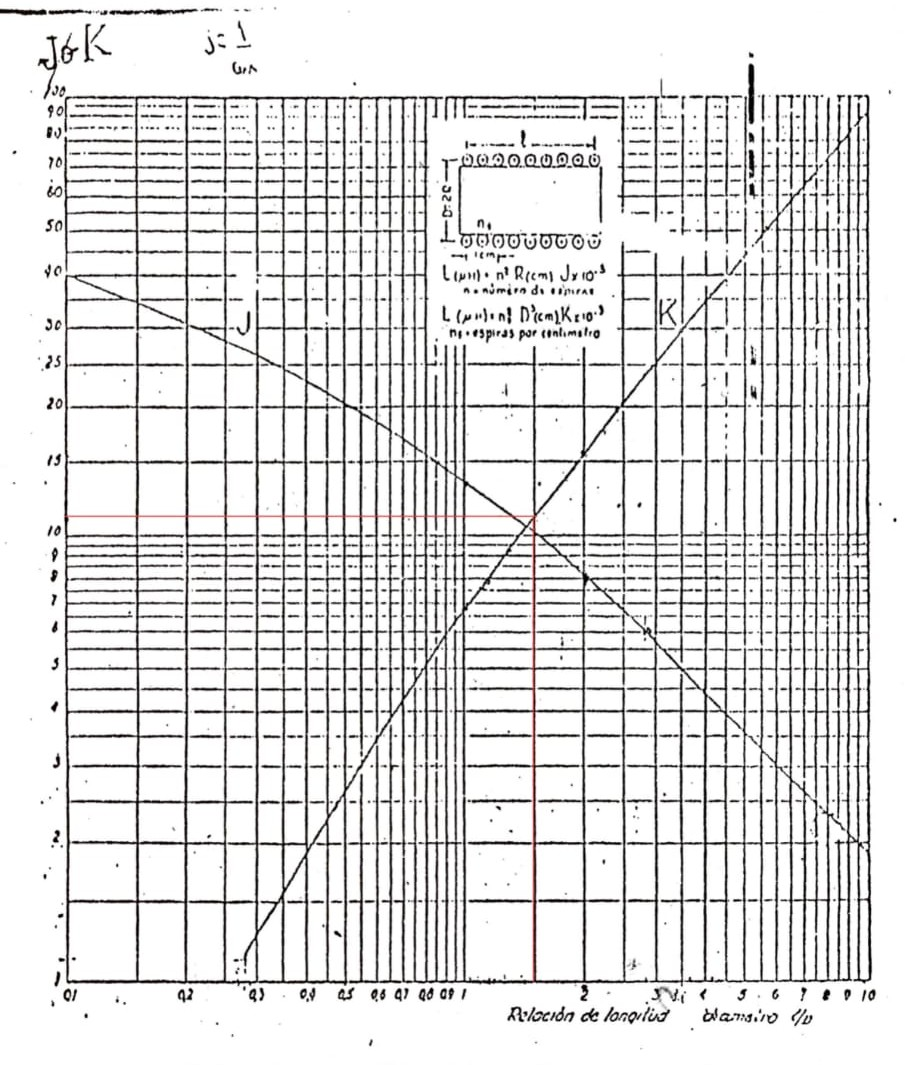
\includegraphics[scale=0.2]{Imagenes/CURVAK.jpeg}
    \caption{Curva K}
    \label{fig:K}
\end{figure}

Se calculan las variables faltantes:

\begin{equation}
    N_s =\frac{1}{0,1cm+0,1cm} = 5 \,\ \frac{v}{cm}
\end{equation}
Si bien \(N_s\) se requiere para calcular el valor del inductor, también se necesita saber cuantas vueltas tiene este para su construcción:
\begin{equation}
    N = N_s \ell = 5\frac{v}{cm}\times3cm = 15 \,\ vueltas
\end{equation}
Finalmente, se calcula la inductancia \(L\) mediante la ecuación (11):
\begin{equation}
    L = 2^3 \times 5^2 \times 11,5 \times 10^{-3} = 2,3\,\ \mu \text{Hy}
\end{equation}

\subsection{Cálculo de \(R_p\) y \(R_T\) }

Si se observa la ecuación (2), falta una variable de calcular para poder despejar \(R_p\). Dicha variable es \(Q_d\), la cual se calcula de la siguiente forma:
\begin{equation}
    Q_d = 8850\frac{D\ell}{102\ell+45D}\sqrt{f_o} = 8850\frac{2\cdot3}{102\cdot3+45\cdot2}\sqrt{14} = 501,72
\end{equation}
Luego, se despeja la ecuación (2) para obtener  \(R_p\):

\begin{equation}
    R_p = Q_dX_L = 501,72 \cdot 2\pi \cdot14\cdot 2,3 \cdot 10^{-6} = 101507,72 \Omega
\end{equation}


La resistencia \(R_T\) se despeja de la ecuación (3) sabiendo que \(BW = 1,4MHz\):
\begin{equation}
    R_T = \frac{f_o}{BW}X_L = \frac{14}{1,4}\cdot2\pi \cdot14\cdot 2,3 = 2023,19 \Omega
\end{equation}
\newpage
\subsection{Cálculo de \(R_a'\) y \(R_L'\)}
Para calcular \(R_a'\), se utiliza la ecuación (9):
\begin{equation}
    R_a' = 2\cdot R_T = 2 \cdot 2023,19\Omega = 4046,38 \Omega
\end{equation}
De igual manera con \(R_L'\) se utiliza la ecuación (8):
\begin{equation}
    R_L' = \frac{2\cdot R_TR_p}{R_p-2R_T} =  \frac{2\cdot 2023,19 \cdot 101507,72}{101507,72-2\cdot 2023,19} = 4214,37 \Omega
\end{equation}

\subsection{Cálculo de Capacitores}
Para el calculo de los capacitores, en primer lugar, se debe determinar la capacidad total \(C_T\), la cual se calcula mediante la ecuación (1):
\begin{equation}
    C_T = (\frac{1}{2\pi f_o\sqrt{L}})^2 = (\frac{1}{2\pi\cdot 14\cdot10^6\sqrt{2,3\cdot10^-6}})^2 = 56,19 \,\ pF
\end{equation}

Lo siguiente, es calcular los capacitores \(C_1, C_2, C_3 y C_4 \). Para ello se utilizarán las ecuaciones (5) y (6) para despejar los valores de dichos capacitores.
\begin{equation}
    C_2 = \frac{C_T}{2}\sqrt{\frac{R_a'}{R_a}} = \frac{C_T}{2}\sqrt{\frac{2R_T}{R_a}} = \frac{56,19pF}{2}\sqrt{\frac{2\cdot2023,19\Omega}{50\Omega}} = 272,74 \,\ pF
\end{equation}

\begin{equation}
    C_1 = \frac{C_2}{\sqrt{\frac{R_a'}{R_a}-1}} = \frac{272,74pF}{\sqrt{\frac{4046,38\Omega}{50\Omega}-1}} = 31,6 \,\ pF
\end{equation}

\begin{equation}
    C_4 = \frac{C_T}{2}\sqrt{\frac{R_L'}{R_L}} = \frac{C_T}{2}\sqrt{\frac{2R_TR_p}{R_L(R_p-2R_T)}} = \frac{56,19pF}{2}\sqrt{\frac{2\cdot2023,19\Omega \cdot 101507,72\Omega}{1000\Omega(101507,72\Omega-2\cdot2023,19\Omega)}} = 57,67 \,\ pF
\end{equation}

\begin{equation}
    C_3 = \frac{C_4}{\sqrt{\frac{R_L'}{R_L}-1}} = \frac{57,67pF}{\sqrt{\frac{4214,37\Omega}{1000\Omega}-1}} = 54,77 \,\ pF
\end{equation}





\newpage
\section{Simulaciones}
\subsection{Simulación con valores teóricos}
Se simuló el circuito con todos los componentes calculados:
\begin{figure}[!h]
    \centering
    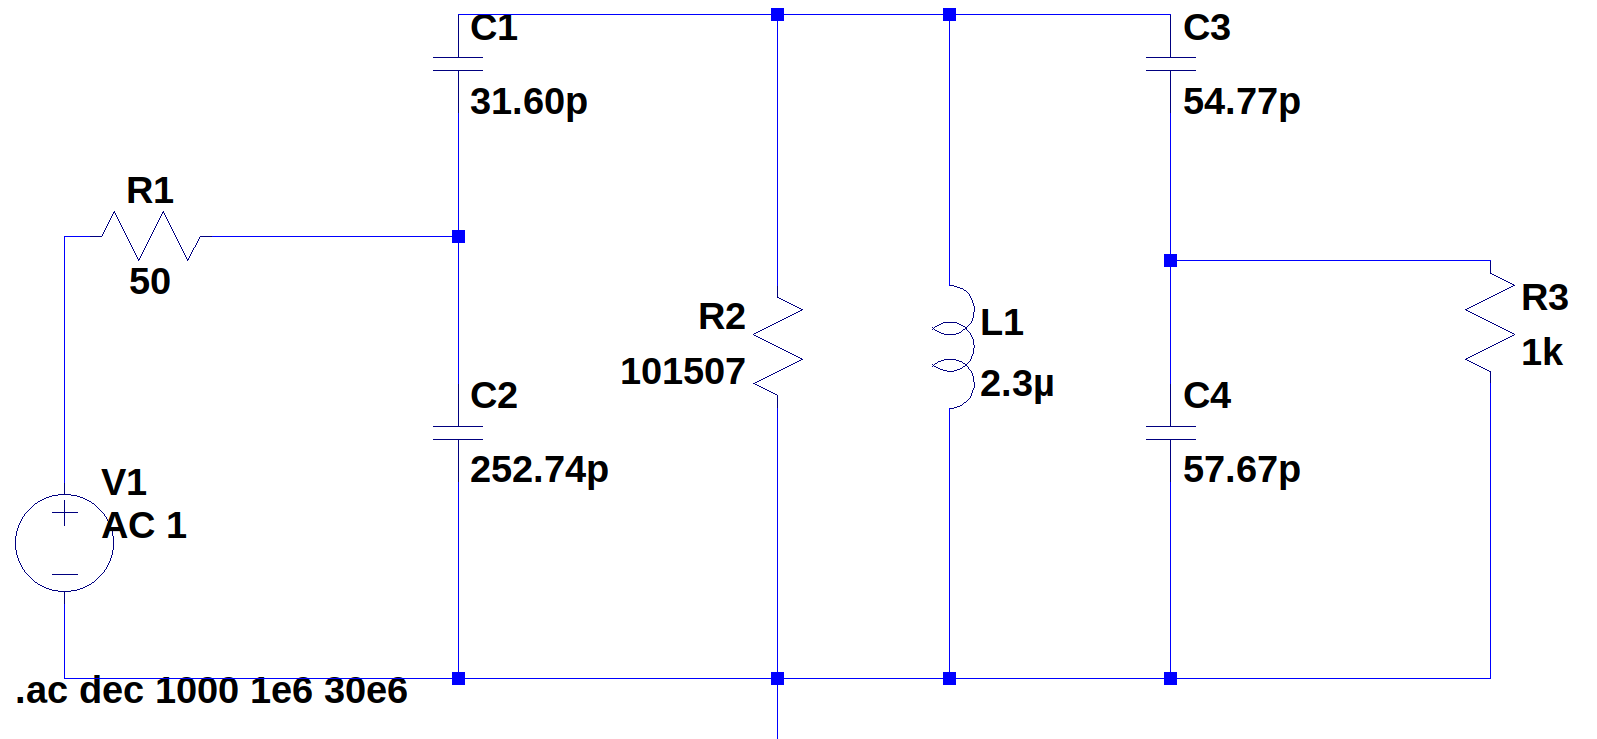
\includegraphics[scale=0.2]{Imagenes/Circuito teorico.png}
    \caption{Esquemático del circuito teórico en LTspice}
    \label{fig:Circteo}
\end{figure}

\begin{figure}[!h]
    \centering
    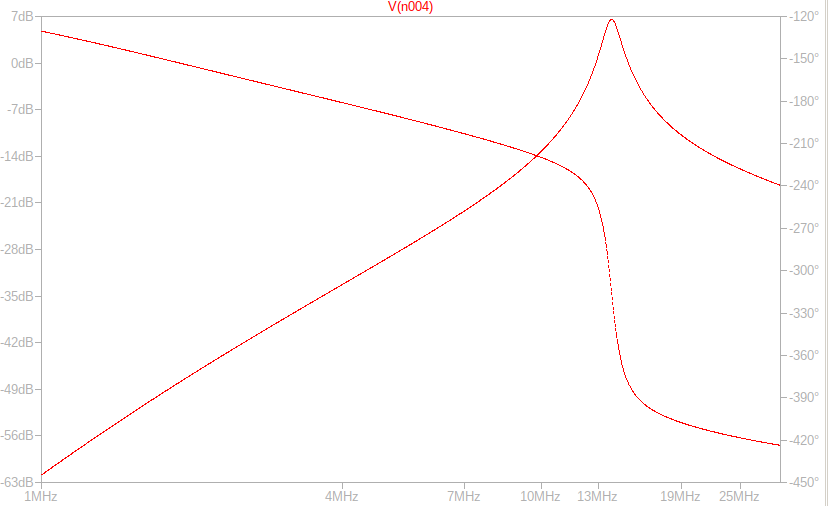
\includegraphics[scale=0.4]{Imagenes/db_f.png}
    \caption{Diagrama de Bode de amplitud y fase}
    \label{fig:Circteo}
\end{figure}

\newpage
\begin{figure}[!h]
    \centering
    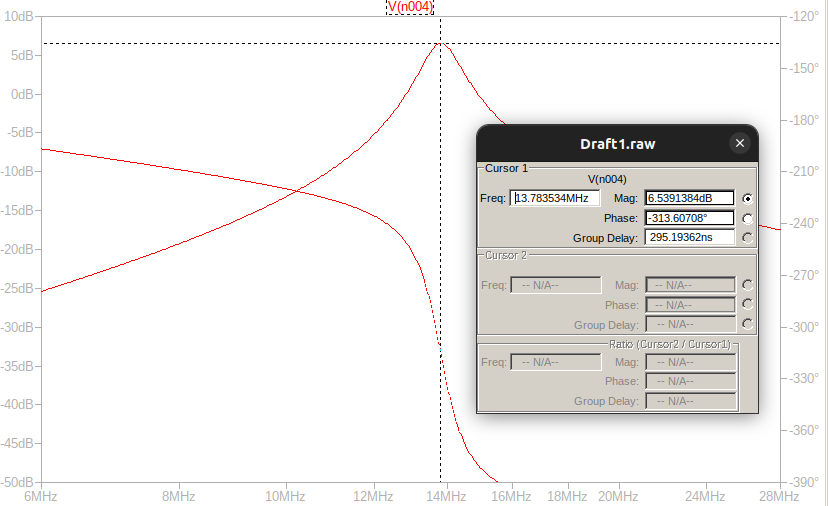
\includegraphics[scale=0.4]{Imagenes/dbzoom.png}
    \caption{Diagrama de Bode ampliado en \(f_o\)}
    \label{fig:Circteo2}
\end{figure}
Se observa que la frecuencia \(f_0\) es aproximadamente 13,78 MHz y se tiene una amplitud de 6,53 dB. Lo siguiente es medir su \(BW\) donde la amplitud caiga 3 dB :
\begin{figure}[!h]
    \centering
    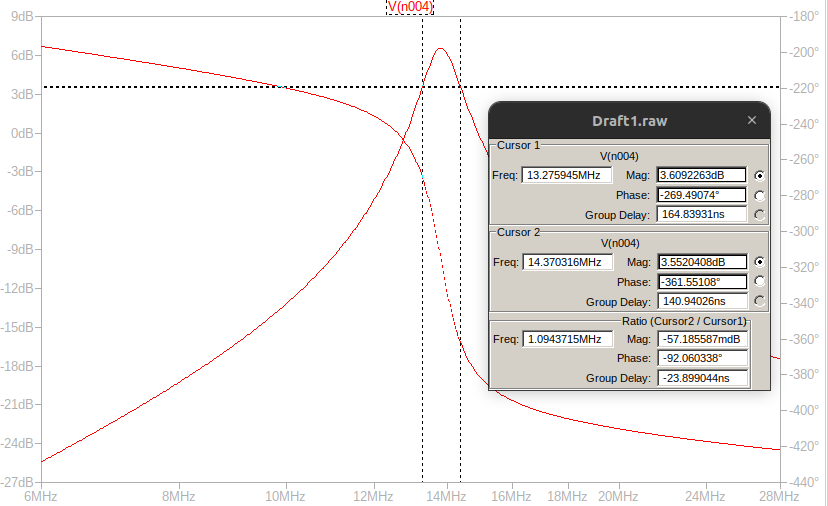
\includegraphics[scale=0.4]{Imagenes/BW.png}
    \caption{Medición del \(BW\)}
    \label{fig:bw}
\end{figure}

Si se observa la figura 12, de esta se puede extraer que el \(BW = 1,1\) MHz aproximadamente. 
\newpage
\subsection{Simulación con valores de capacitores comerciales conseguidos.}
Para los valores comerciales que se pudieron conseguir, se simuló el circuito con dichos valores de capacitores para observar como variaba la \(f_o\):
\begin{figure}[!h]
    \centering
    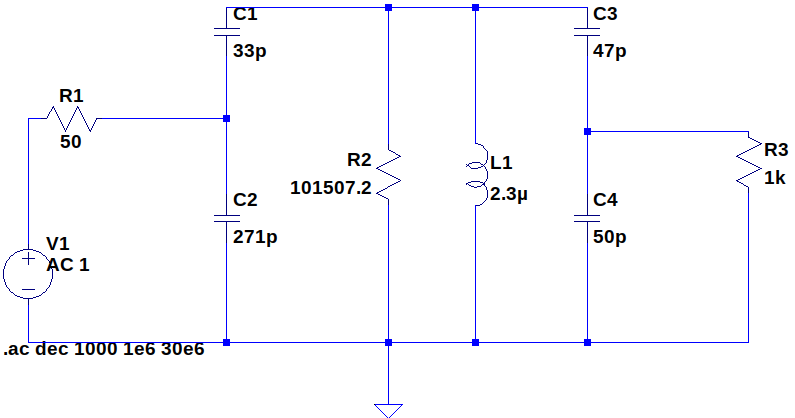
\includegraphics[scale=0.4]{Imagenes/Circreal.png}
    \caption{Esquemático de circuito con capacitores comerciales}
    \label{fig:bw}
\end{figure}

\begin{figure}[!h]
    \centering
    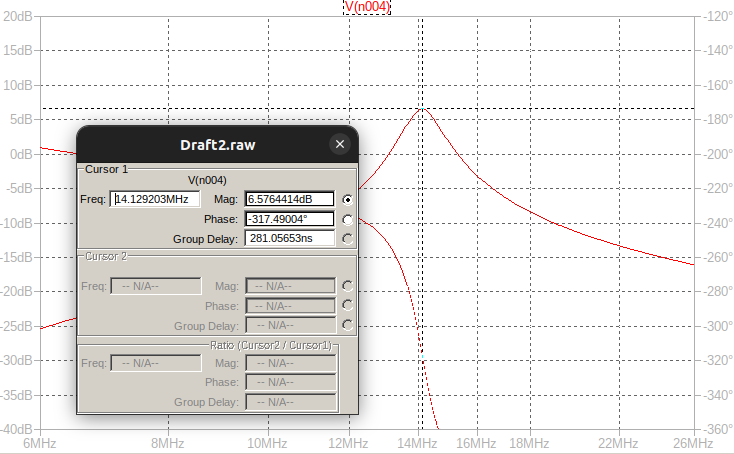
\includegraphics[scale=0.4]{Imagenes/Circreal_bode.png}
    \caption{Diagrama de Bode }
    \label{fig:bw}
\end{figure}
La frecuencia de resonancia central \(f_o\) es 14,13 MHz, la amplitud y el \(BW\) son prácticamente los mismos. Por ultimo, se calcula el \(Q_c\) mediante la ecuación (3): 
\begin{equation}
    Q_c = \frac{14,13 \text{MHz}}{1,1 \text{MHz}} = 12,84 
\end{equation}



\newpage
\section{Circuito construido}
\subsection{Componentes utilizados}
El circuito que se construyó es el de la figura 13, para su implementación física, se utilizaron los siguientes componentes:
\begin{itemize}
    \item Placa de fenólico simple faz 5x5.
    \item 2 BNC hembra
    \item Alambre de cobre esmaltado de 1 mm de diámetro
    \item \(C_1 = 33\) pF
    \item \(C_2 = 271\) pF
    \item \(C_3 = 47\) pF
    \item \(C_4 = 50\) pF (Se utilizaron dos capacitores en serie de 100 pF)
    \item \(R_L = 1\) k\(\Omega\)
\end{itemize}
\begin{figure}[!h]
    \centering
    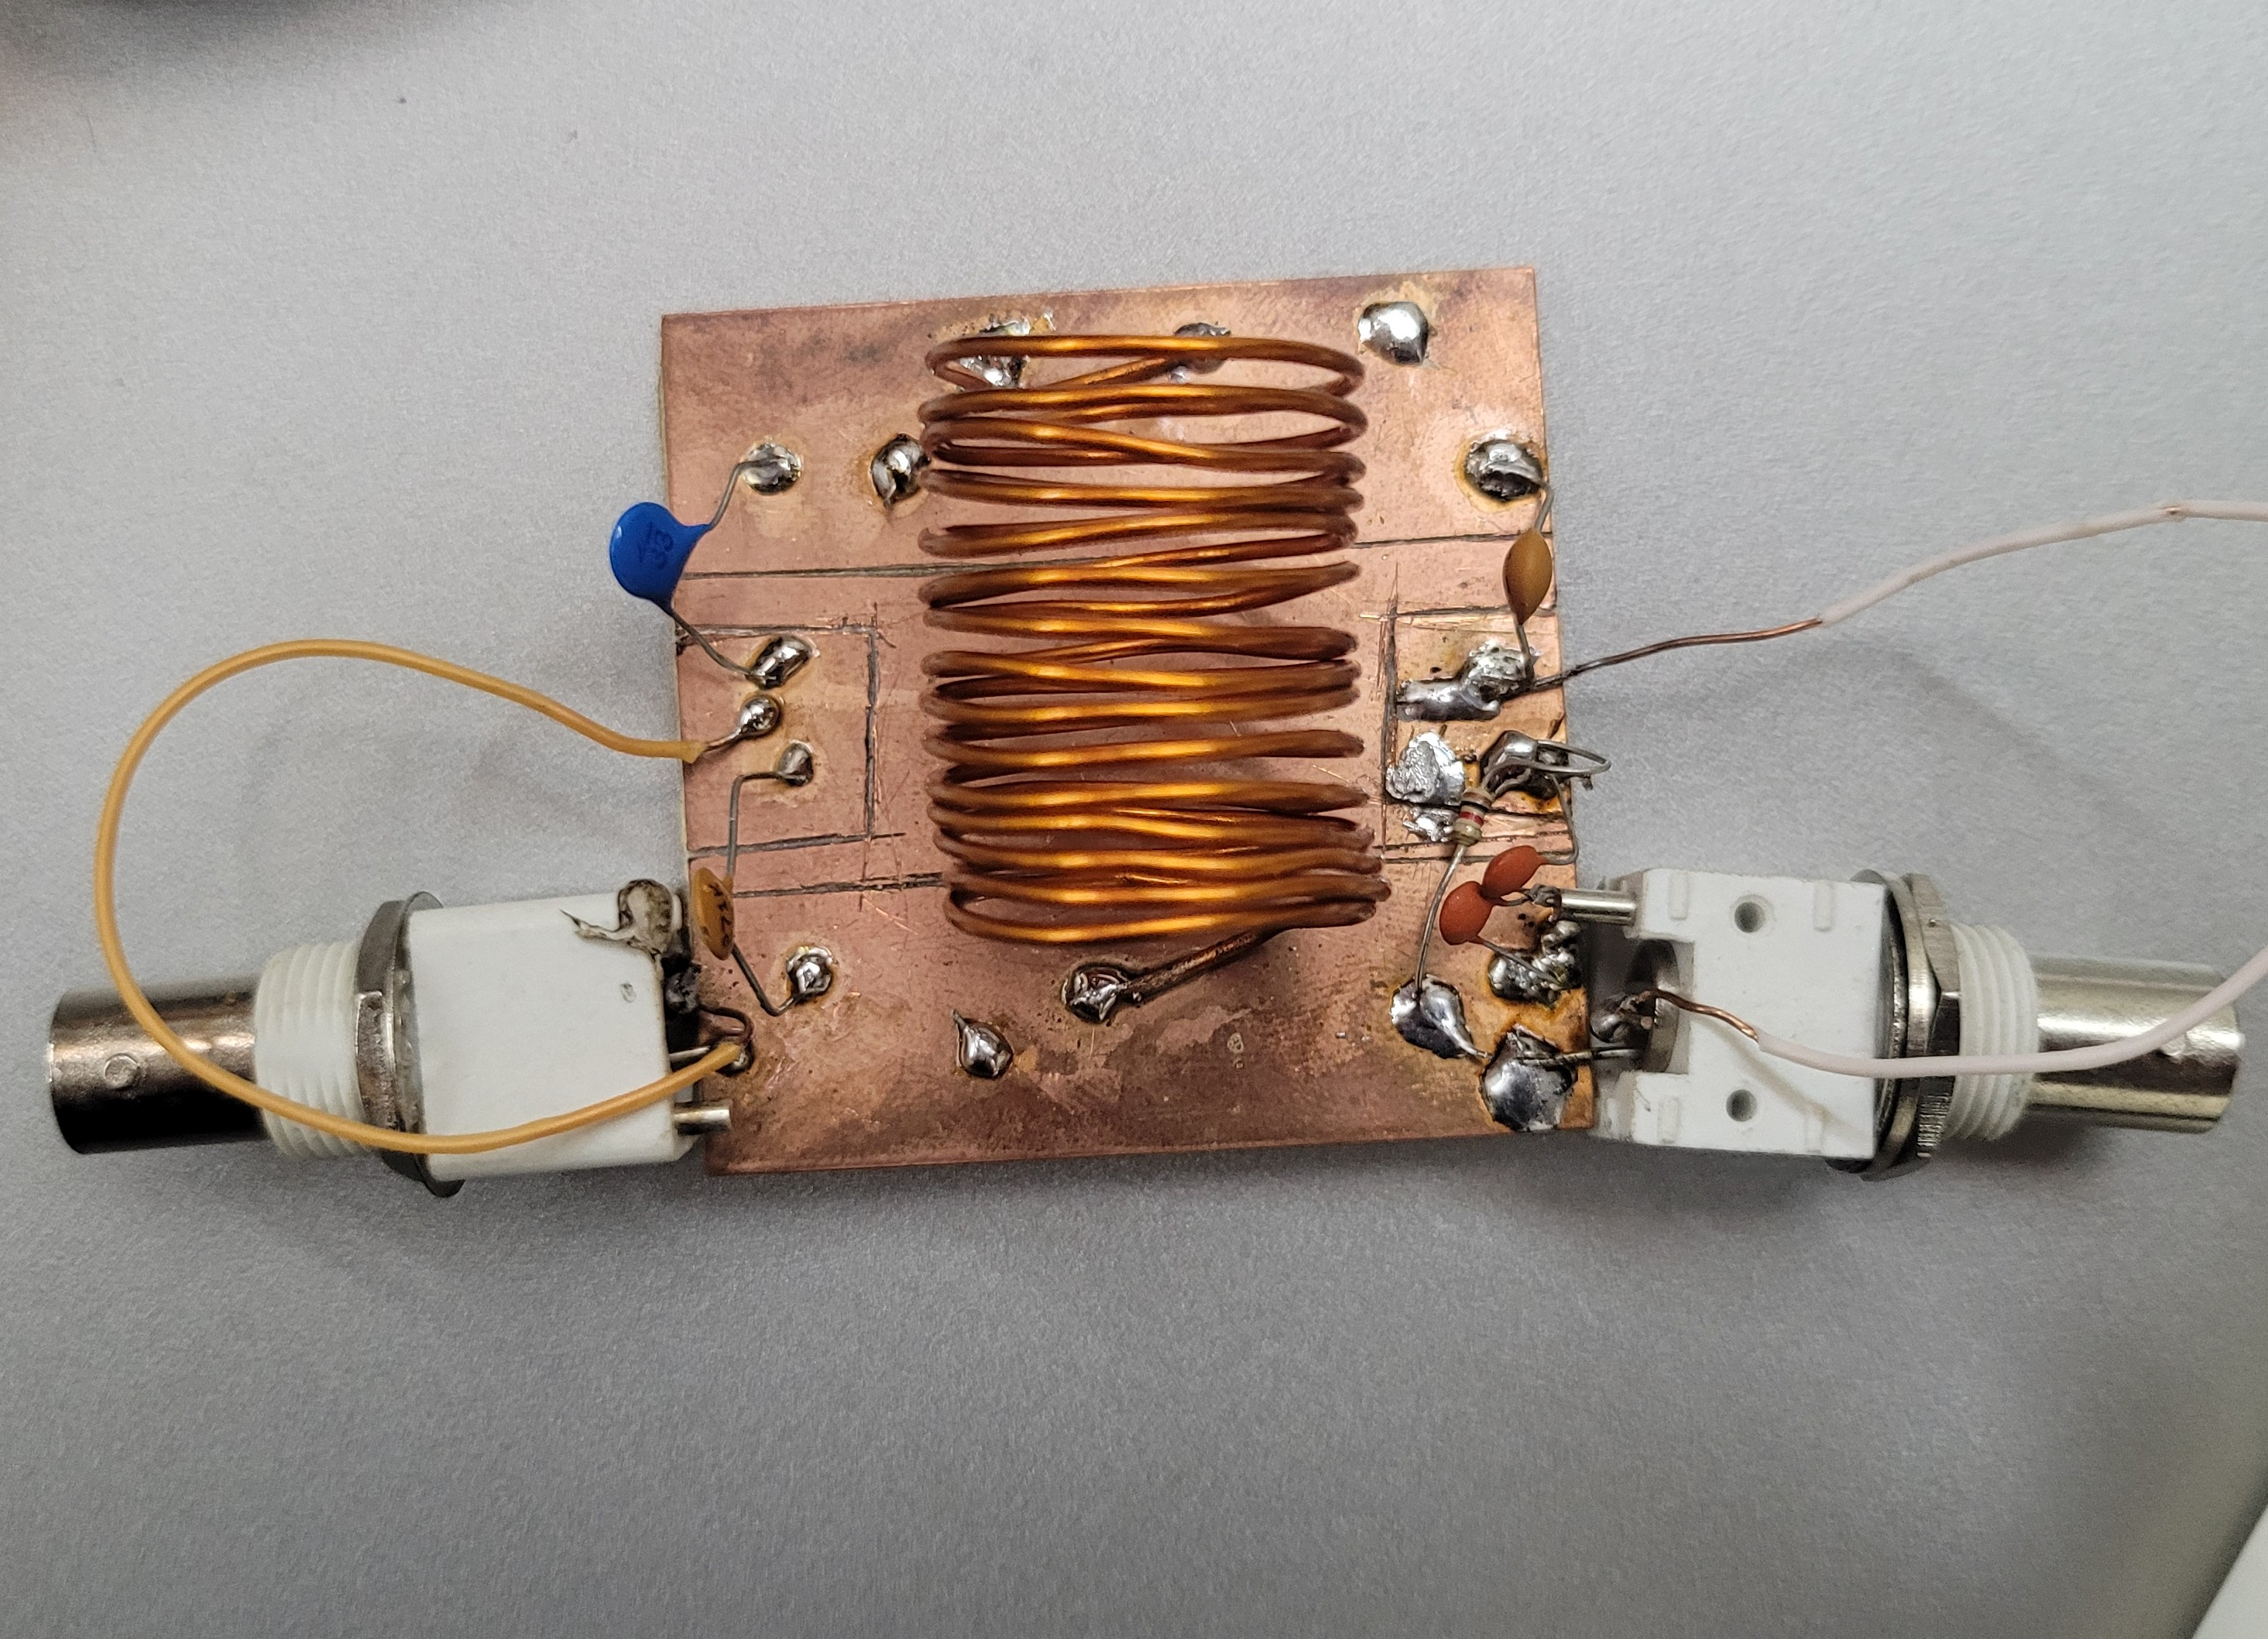
\includegraphics[scale=0.1]{Imagenes/Circuito montado.jpg}
    \caption{Circuito construido}
    \label{fig:Circteo__}
\end{figure}
Se calculó la capacidad total de la siguiente forma:
\begin{equation}
    C_T = (C_1//C_2)+(C_3//C_4) = 29,44pF + 24,22pF = 53,66 \,\ \text{pF}
\end{equation}

\newpage
\subsection{Mediciones}
\subsubsection{Circuito conectado a tope}
\begin{figure}[!h]
    \centering
    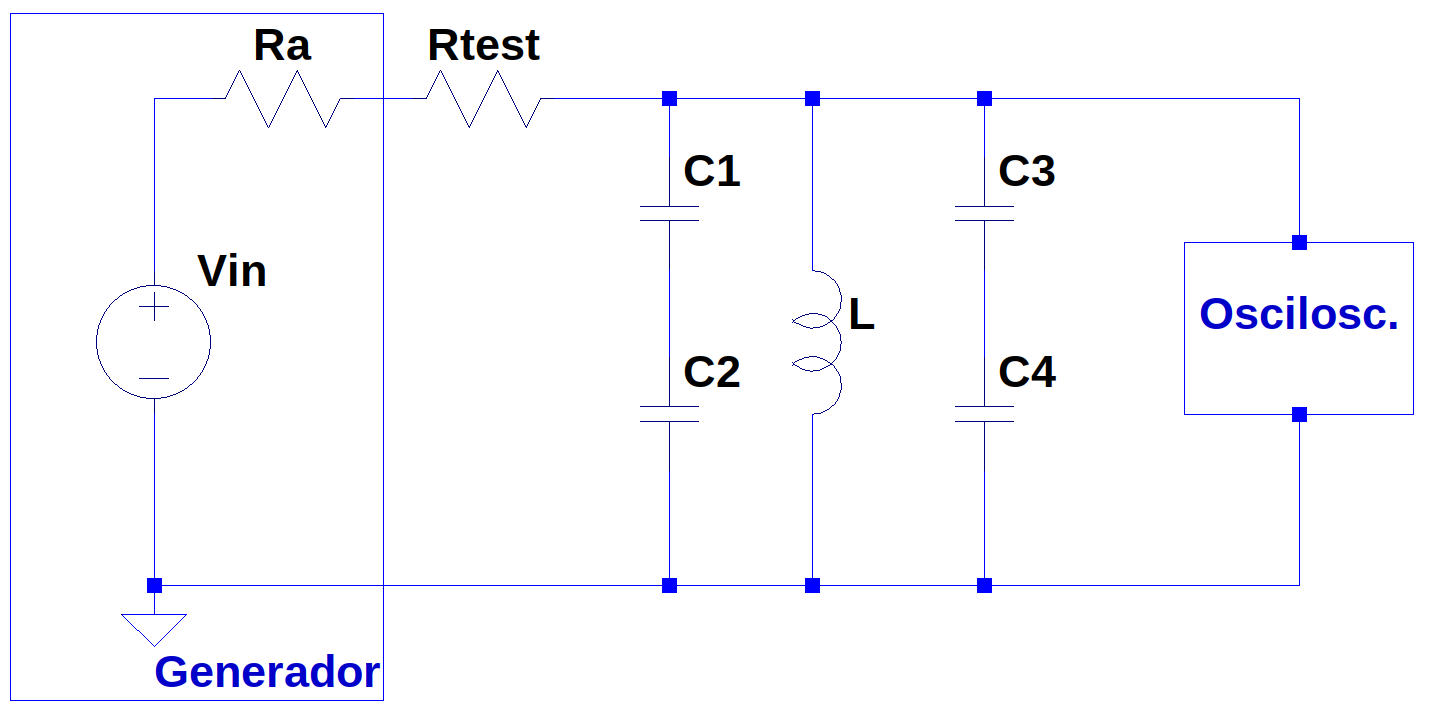
\includegraphics[scale=0.3]{Imagenes/Circuito conectado a tope.png}
    \caption{Circuito conectado a tope}
    \label{fig:Circtope}
\end{figure}
Para esta configuración se agrega \(R_t_e_s_t = 1\)k\(\Omega\) y los instrumentos se conectaron como se observa en la figura 16.
En este tipo de conexión, se realizaron 3 mediciones: \(f_o_1\), \(f_o_2\), \(R_p\).

La \(f_o\) no es posible medirla de manera directa debido a todas las capacidades parásitas que se agregan al circuito al realizar las mediciones, tanto los conectores, cables y el mismo osciloscopio agregan capacidades al circuito que afectan la capacidad total del circuito y esto modifica la frecuencia de resonancia del mismo. El método que se utilizó para calcular \(f_o\) es despejarlo a partir de  las dos mediciones \(f_o_1\) y \(f_o_2\)\ %mediante la medicion de dos frecuencias de resonancias, \(f_o_1\) tal como se observa en la figura 12 y \(f_o_2\) agregando un capacitor conocido \(C_F\) en paralelo a la bobina, el cual es de 18 pF.

Para medir la \(f_o_1\), se buscó el valor donde resonaba el circuito, es decir, donde su amplitud en tensión era máxima:
\begin{equation}
    f_o_1 = 7,8 \,\ \text{MHz} 
\end{equation}

En esta misma medición, se observo que amplitudes se tenían, la del generador y la señal que mide el osciloscopio a la salida del circuito:

\begin{align}
    V_{\mathrm{gen}} &= 3.64 \, \mathrm{V_{pp}} \\
    V_{\mathrm{out}} &= 3.40 \, \mathrm{V_{pp}}
\end{align}

Luego, para la medición de \(f_o_2\) se agregó un capacitor \(C_F = 18\) pF en paralelo a la bobina para con esto modificar la frecuencia de resonancia:

\newpage
\begin{figure}[!h]
    \centering
    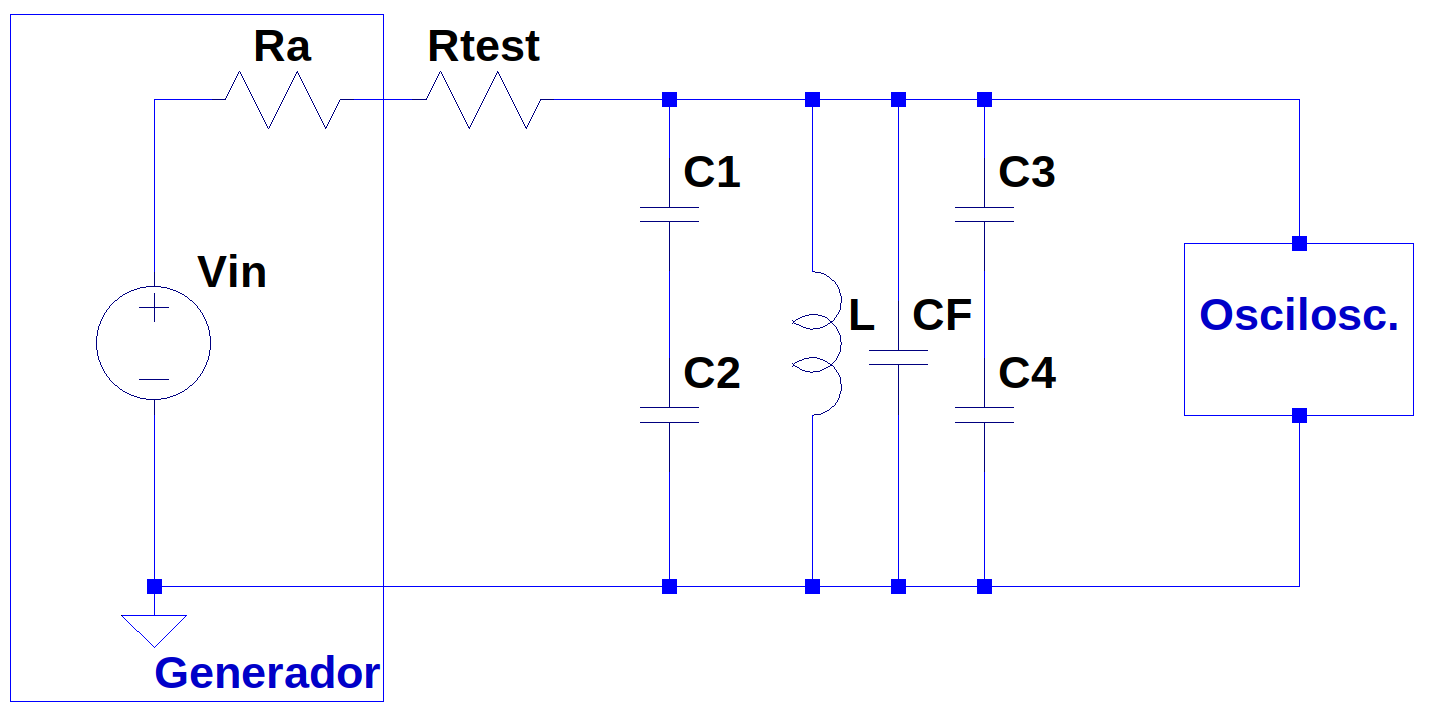
\includegraphics[scale=0.3]{Imagenes/CF.png}
    \caption{Capacitor \(C_F\) en paralelo a la bobina}
    \label{fig:Circtope}
\end{figure}
Se buscó nuevamente la frecuencia de resonancia con esta modificación y se obtuvo:
\begin{equation}
    f_o_2 = 7,43 \,\ \text{MHz} 
\end{equation}

Por lo tanto, lo siguiente fue encontrar las capacidades parásitas \(C_X\), el cual se encuentra en paralelo en ambos circuitos. Para ello, se utiliza la ecuación (1):

\begin{equation}
    f_o_1 = \frac{1}{2\pi \sqrt{(C_T+C_X)L}} = 7,8 \,\ \text{MHz}
\end{equation}

\begin{equation}
    f_o_2 = \frac{1}{2\pi \sqrt{(C_T+C_X+C_F)L}} = 7,43 \,\ \text{MHz}
\end{equation}
\begin{gather}
    \left(\frac{f_{o1}}{f_{o2}}\right)^2 = \frac{(2 \pi)^2 (C_T+C_X+C_F)L}{(2 \pi)^2 (C_T+C_X)L} \notag \\
    \left(\frac{f_{o1}}{f_{o2}}\right)^2 = \frac{C_T+C_X+C_F}{C_T+C_X} \notag \\
    \hspace{2.5em} C_X\left[\left(\frac{f_{o1}}{f_{o2}}\right)^2-1\right]+C_T\left(\frac{f_{o1}}{f_{o2}}\right)^2 =C_T+C_F \notag \\
    C_X =\frac{C_T((f_o_2)^2-(f_o_1)^2)+C_F (f_o_2)^2}{(f_o_1)^2-(f_o_2)^2} \label{eq:conjunto}
\end{gather}
Reemplazando se obtuvo:
\begin{equation}
    C_X = 122,68 \,\ \text{pF}
\end{equation}

Se utilizó la ecuación (32) para despejar L:

\begin{equation}
    L = \frac{1}{(2\pi\cdot7,8\text{MHz})^2}\cdot\frac{1}{53,66pF+122,68pF} = 2,36 \,\ \mu\text{Hy}
\end{equation}

\newpage

Con \(L\), se tienen todos los valores necesarios para calcular la frecuencia de resonancia.

\begin{equation}
    f_o = \frac{1}{2\pi \cdot \sqrt{LC}} = \frac{1}{2\pi \cdot \sqrt{2,36\mu \text{Hy}\cdot 53,6\text{pF}}} = 14,14 \,\ \text{MHz}
\end{equation}

Finalmente, queda calcular \(R_p\), este se calcula a partir de los valores de tensión obtenidos en la medición de \(f_o_1\), el circuito equivalente de análisis es el siguiente:

\begin{figure}[!h]
    \centering
    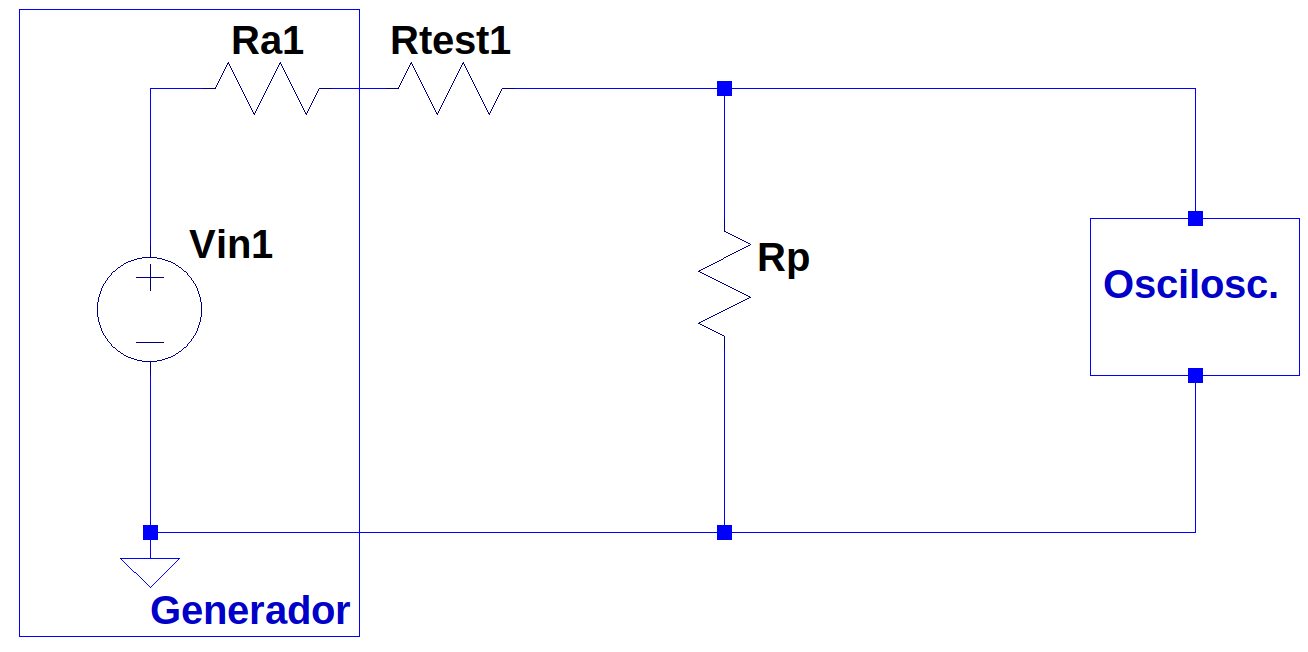
\includegraphics[scale=0.3]{Imagenes/RP.png}
    \caption{Circuito equivalente para medir \(R_p\)}
    \label{fig:Circrp}
\end{figure}

Se plantea un divisor de tensión, del cual se despeja \(R_p\):
\begin{equation}
    V_o_u_t = V_g_e_n\frac{R_p}{R_p+R_a+R_t_e_s_t} 
\end{equation}
De la ecuación (29) y (30) se utilizaran los valores de tensión.
\begin{equation}
    3,40V = 3,64V\frac{R_p}{R_p+50\Omega+1k\Omega} 
\end{equation}

\begin{equation}
    R_p = \frac{R_a+R_t_e_s_t}{(\frac{V_g_e_n}{V_o_u_t})-1} = \frac{50\Omega+1k\Omega}{(\frac{3,64V}{3,40V})-1} = \boxed{14,88 \,\ k\Omega}
\end{equation}

Con \(R_p\) se calcula \(Q_d\):

\begin{equation}
    Q_d = \frac{R_p}{X_L} = \frac{14,88k\Omega}{2\pi \cdot 14 \text{MHz} \cdot 2,3\mu \text{Hy}} = \boxed{73,54} 
\end{equation}

\newpage

\subsubsection{Circuito conectado al punto medio}

\begin{figure}[!h]
    \centering
    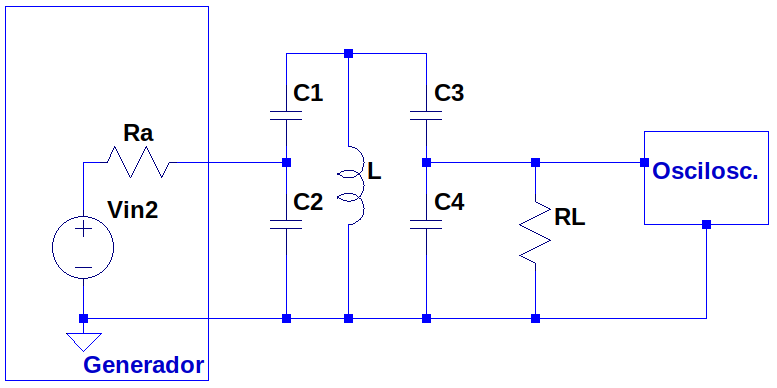
\includegraphics[scale=0.4]{Imagenes/Circptomedio.png}
    \caption{Circuito conectado al punto medio}
    \label{fig:Circrp}
\end{figure}

Para esta configuración se desconecto \(R_t_e_s_t\) y se conectó \(R_L\). Como también las conexiones del generador y osciloscopio se conectaron de la forma que se observa en la figura 19.

En esta configuración se realizaron todas las mediciones faltantes: \(BW\), \(Z_i_n\), \(Z_o_u_t\), \(Q_c\).

Para la medición de \(BW\) se buscó la resonancia del circuito, la cual, como es de esperar, es una frecuencia de resonancia distinta a las anteriores. Por lo tanto, se realizó un barrido en frecuencia hasta encontrar el valor de tensión máximo:


\begin{equation}
    V_o_u_t = 3,88 \,\ V_p_p
\end{equation}

\begin{equation}
    f_o_4 = 12,13 \,\ \text{MHz}
\end{equation}



Luego, se buscaron los valores de tensión para los cuales caen 3 dB lo que es equivalente a la siguiente ecuación:
\begin{equation}
    V_f_c = 3,88 \,\ V_p_p \cdot 0,707 = 2,74 \,\ V_p_p
\end{equation}

Por lo tanto, se buscó la frecuencia de corte superior e inferior para dicho valor de tensión.

\begin{equation}
    f_c_l = 11,95 \,\ \text{MHz}
\end{equation}

\begin{equation}
    f_c_h = 12,39 \,\ \text{MHz}
\end{equation}

Con los valores encontrados de frecuencia, se calculó el BW:

\begin{equation}
BW = 12,39 - 11,95 = \boxed{0,44 \,\ \text{MHz}}
\end{equation}

Con \(BW\) se calculó \(Q_c\) con la ecuación (3):
\begin{equation}
    Q_c= \frac{14,14 \,\ \text{MHz}}{0,44 \,\ \text{MHz}} = \boxed{32,13}
\end{equation}

\newpage
La siguiente medición es \(Z_i_n\), para lo cual, se van a medir valores de tensión a la entrada, la disposición es la siguiente:

\begin{figure}[!h]
    \centering
    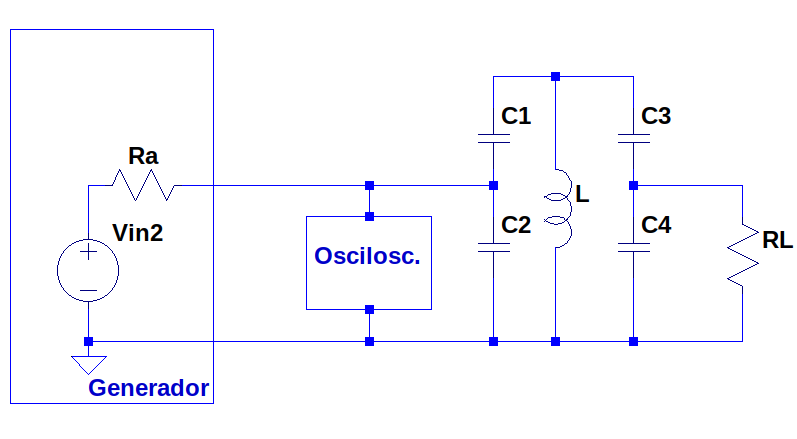
\includegraphics[scale=0.4]{Imagenes/ZIN.png}
    \caption{Medición de \(Z_i_n\)}
    \label{fig:Zin}
\end{figure}

De esta forma, la medición consiste en observar como cae la tensión del generador al conectar el circuito como se observa en la figura 20, si este cae a la mitad, el circuito se encontraría adaptado:

\begin{equation}
    V_g_e_n = 3,28 \,\ V_p_p
\end{equation}

Luego, se mide la caída de tensión:

\begin{equation}
    V_o_s_c = 1,32 \,\ V_p_p
\end{equation}

\begin{equation}
   V_o_s_c  = V_g_e_n \cdot \frac{Z_i_n}{Z_i_n+R_a} 
\end{equation}

Despejando \(Z_i_n\) de la ecuación (51):
\begin{equation}
    Z_i_n = R_a \frac{V_o_s_c}{V_g_e_n-V_o_s_c} = 50\Omega \frac{1,32V}{3,28V-1,32V} = \boxed{33,67 \Omega}
\end{equation}

\newpage
La siguiente medición es \(Z_o_u_t\), para la cual se deben realizar dos mediciones. Una medición se realizó como esta dispuesto en la figura 19, que es la medición con el circuito cargado y luego otra medición es desconectando la carga \(R_L\), es decir, descargado.

\begin{figure}[!h]
    \centering
    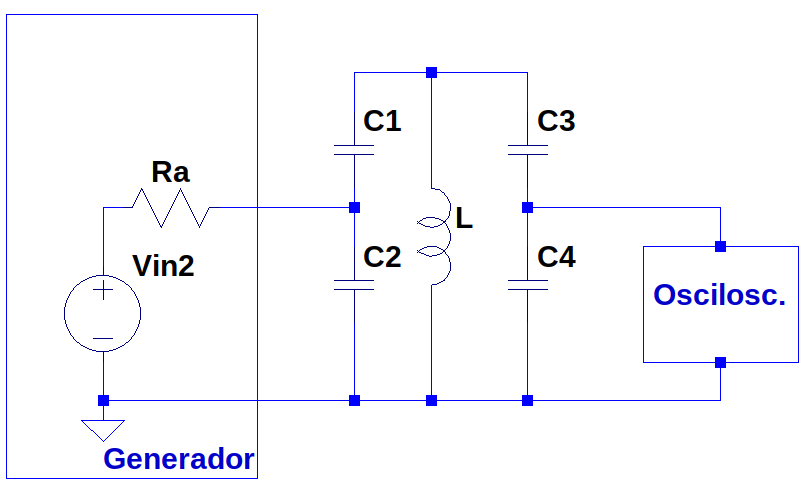
\includegraphics[scale=0.4]{Imagenes/Zout.png}
    \caption{Medición de \(Z_o_u_t\) descargado}
    \label{fig:Zin}
\end{figure}

Los valores que se obtuvieron del osciloscopio son las tensiones, por un lado la tensión de salida con el circuito cargado \(V_L\) y con el circuito descargado \(V_o_u_t\).

\begin{equation}
    V_L = 5,84 V
\end{equation}

\begin{equation}
    V_o_u_t = 6,96 V
\end{equation}

Luego, se plantea un divisor de tensión similar al que se planteó en la ecuación (51)

Por lo que se calcula \(Z_o_u_t\) de la siguiente manera:

\begin{equation}
    Z_o_u_t = R_L \frac{V_o_u_t-V_i_n}{V_L} = 1k\Omega\frac{6,96V-5,84V}{5,84V} = \boxed{191,78\Omega}
\end{equation}



\newpage
\section{Comparación de resultados}
Se realizó una tabla comparativa de los resultados para luego analizar el origen de las discrepancias entre ellas.

\begin{table}[h]
\centering
\begin{tabular}{|c|c|c|c|c|c|}
\hline
Parámetros & Unidades & Teórico & Simulado & Medido & ERP \\
\hline
\(L\)  & \mu Hy & 2,3 & 2,3 & 2,36 & 10,43\% \\
\hline
\(C_T\)& pF & 56,19 & 53,66 & 53,66 &  \\
\hline
\(f_o\)& MHz & 14 & 14,13 & 14,14 & 1\% \\
\hline
\(BW\)& MHz & 1,4 & 1,1 & 0,44 & 68,57\%\\
\hline
\(Q_c\)&  & 10 & 12,84 & 32,13 & 221,3\%\\
\hline
\(Q_d\)&  & 501,72 & 501,72 & 73,54 & 85,35\% \\
\hline
\(R_p\)& k\Omega  & 101,5 & 101,5 & 14,88 & 85,33\%\\
\hline
\(Z_i_n\)& \Omega  & 50 &  & 33,67 & 32,66\%\\
\hline
\(Z_o_u_t\)& \Omega  & 1000 &  & 191,78 & 80,82\% \\
\hline
\end{tabular}
\caption{Comparación de resultados}
\label{tab:mi_tabla}
\end{table}
Siendo ERP el error relativo porcentual entre el valor teórico y el valor medido, tomando como valor real al teórico.

\newpage
\section{Conclusión}
Se pudo realizar el trabajo practico, en el cual se aplicaron los conceptos vistos en clase como también conceptos vistos en materias anteriores, a su vez, se obtuvieron diferencias entre lo medido y la calculado de manera teórica, a continuación se analizan estas cuestiones:
\begin{itemize}
    \item Se pudo pudo diseñar el inductor de manera teórica y luego implementarlo físicamente, el cual a pesar de presentar discrepancias físicas respecto a su diseño ideal, el valor medido es prácticamente igual al calculado de manera teórica. Sin embargo el inductor no es ideal y sus resistencias de pérdidas \(R_p\) es aproximadamente un 15\% del valor teórico, por lo tanto, la corriente que circulara por esta resistencia será mayor lo cual genera pérdidas y hace menos eficiente el inductor, por lo tanto es de esperar que esto disminuya en igual proporción a \(Q_d\), pero a su vez, si se analiza la ecuación (20) se observa que \(R_L'\) depende de \(R_p\), se reescribe dicha ecuación para poder observar de manera mas intuitiva como afecta \(R_p\):
    \begin{equation}
    R_L' = \frac{2\cdot R_TR_p}{R_p-2R_T} =  \frac{2R_T}{1-2\frac{R_T}{R_p}}
\end{equation}
Es evidente que, lo ideal seria que \(R_p\) tienda a infinito, de esta forma se cumpliría que el paralelo de \(R_a'\) y \(R_L'\) es igual a \(R_T\). Esto afecta directamente en las adaptaciones de salida como en la de entrada, como pudo observarse en las mediciones realizadas. Las capacidades de los instrumentos, conectores, etc. también afectaron directamente en la adaptación de dichas impedancias, como se pudo observar cuando se realizaron dichas mediciones, las capacidades parásitas eran mayores a 100 pF.
    \item La frecuencia de resonancia central \(f_o\) es la esperada, de hecho esta se corresponde con la simulada, la cual tiene en cuenta los capacitores reales utilizados. Sin embargo, el ancho de banda es mucho más restringido de lo que debería, lo que a su vez provoco un \(Q_c\) mucho mayor al calculado. Una manera de forzar a que \(BW\) aumente es conectar una resistencia en paralelo a la bobina, para de esta forma disminuir \(R_T\) y con esto el \(Q_c\)
\end{itemize}

Finalmente, se concluye que teniendo en cuenta lo mencionado anteriormente, se podrían mejorar los resultados del circuito hasta cierto punto, debido a que la bobina se realiza a mano y eso agrega cierto error humano, como también el tiempo que demoraría iterar entre correcciones y como se observó el error que agregan los instrumentos que se disponen, si bien existen formas para mejorar el diseño y el rendimiento del circuito, los resultados obtenidos hasta el momento son satisfactorios dentro del alcance y las limitaciones del proyecto.
%\printbibliography
\end{document}